\documentclass{beamer}

\usepackage{amsmath}
\usepackage{booktabs}
\usepackage{tabularx}
\usepackage{rotating}
\usepackage{microtype}
\usepackage{indentfirst}
\usepackage{amssymb}
\usepackage{graphicx}
\usepackage{tikz}
\usepackage{lmodern}
\usepackage[T1]{fontenc}
\usepackage[utf8x]{inputenc}

\usetheme[secheader]{Boadilla}
\usecolortheme{beaver}

% Defining some color scheme
\setbeamercolor*{item}{fg=red}
\defbeamertemplate*{itemize subitem}{default}{\tiny\raise1.5pt\hbox{\donotcoloroutermaths$\blacktriangleright$}}
\setbeamercolor*{block title}{fg=black!30!red,bg=black!20}
\setbeamercolor*{block body}{fg=black,bg=black!10}

\title[SecureIt]{SecureIt}
\author{Luca Bonato, Marco Ziccardi}
\date{Sistemi Ipermediali}
\institute[UniPD]{University of Padua\\
\includegraphics[width=15mm]{img/unipd_logo.pdf}}


\begin{document}

\begin{frame}
\begin{minipage}[l]{.7\textwidth}
~\\[4cm]
\includegraphics[width=3.5cm]{./img/icona.pdf}
\end{minipage}\begin{minipage}[r]{.5\textwidth}
~\\[4cm]
\includegraphics[width=3.5cm]{./img/icona.pdf}
\end{minipage}\\[-6.5cm]
\maketitle
\end{frame}

\begin{frame}
\frametitle{Table of contents}
\tableofcontents
\end{frame}

% INTRODUCTION
\section{Introduzione}
\begin{frame}
\frametitle{Obiettivi dell'applicazione}
\begin{block}{Un dispositivo per sicurezza ad ampio spettro}
Avere in un solo dispositivo \textit{molteplici} funzionalità per monitorare uno spazio privato ed il dispositivo stesso
\end{block}
Altre applicazioni sul mercato offrono solo un monitoraggio parziale:
\begin{itemize}
	\item \textbf{Motion Detector Pro}: solo motion detection
	\item \textbf{Sound Detector}: solo noise detection
	\item \textbf{Surveillance}: motion e sound detection. Non usa accelerometro e tracking

\end{itemize}
...si prova a sfruttare tutte le funzionalità del dispositivo per conoscerne i limiti
\end{frame}

\begin{frame}
\frametitle{Funzionalità offerte}
\noindent\begin{minipage}[c]{.7\textwidth}
\begin{enumerate}
  \item \textbf{Accelerometro}: determinare quando il dispositivo viene mosso
  \item \textbf{Fotocamera}: determinare quando c'è movimento nell'ambiente
  \item \textbf{Microfono}: determinare quando c'è rumore nell'ambiente
  \item \textbf{SMS}: per avvisare l'utente di un'intrusione
  \item \textbf{WiFi-3G-Bluetooth}: per fornire all'utente informazioni più accurate
  \item \textbf{Codice sblocco}: per avere controllo sulla chiusura dell'applicazione
  \item \textbf{Sito web}: in cui poter consultare le informazioni raccolte (audio, immagini, locazione dispositivo)
\end{enumerate}
\end{minipage}\begin{minipage}[c]{.25\textwidth}
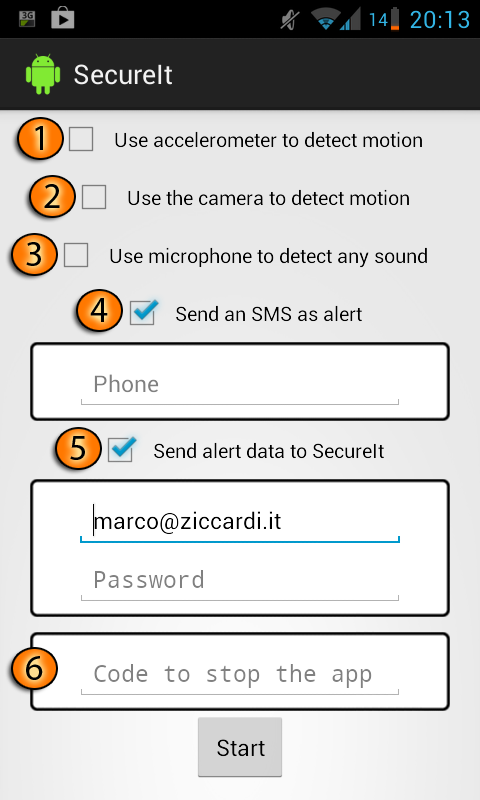
\includegraphics[scale=.2]{./img/firstpage.png}
\end{minipage}
\end{frame}

\section{Rilevamento movimento dispositivo}
\begin{frame}
\frametitle{Accelerometro}
\begin{block}{~}
Attraverso l'accelerometro è possibile determinare quando il dispositivo viene mosso
\end{block}
\begin{itemize}
  \item Un intruso urta per sbaglio il dispositivo
  \item Un intruso prende volontariamente il dispositivo
\end{itemize}

Questa funzionalità viene utilizzata solamente per generare l'allarme
\end{frame}

\begin{frame}
\frametitle{Come viene effettuato}
\begin{minipage}[c]{.7\textwidth}
\begin{itemize}
  \item Possibile determinare la sensibilità (3 valori disponibili) con cui viene riconosciuto il movimento (\texttt{THRESHOLD})
  \item Monitorare per un certo periodo le informazioni offerte dall'accelerometro (accelerazioni sui 3 assi)
        {\footnotesize\[\frac{(\Delta accel_X) + (\Delta accel_Y) + (\Delta accel_Z)}{\Delta t} > \texttt{THRESHOLD}\]}
\end{itemize}
\end{minipage}\begin{minipage}[c]{.25\textwidth}
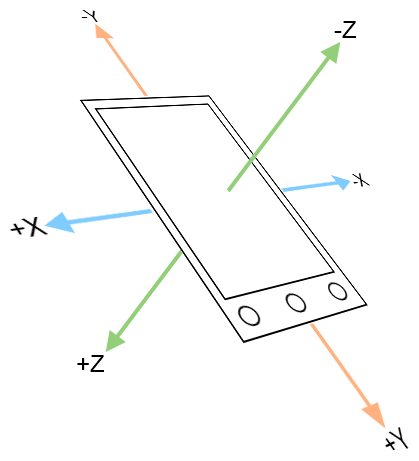
\includegraphics[scale=.3]{./img/accelerometer.png}
\end{minipage}
\end{frame}

\begin{frame}
\frametitle{Cosa viene proposto all'utente}
\begin{minipage}[c]{.25\textwidth}
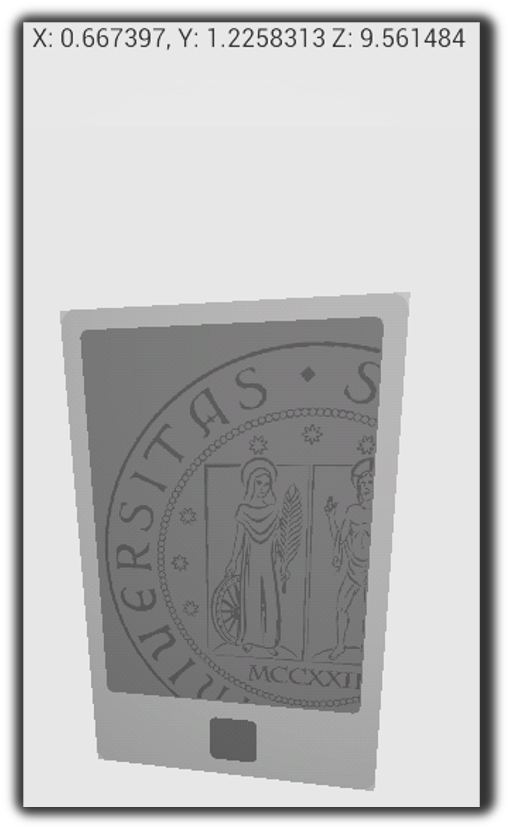
\includegraphics[scale=.18]{./img/opengl.png}
\end{minipage}\begin{minipage}[r]{.65\textwidth}
\begin{itemize}
  \item Schermata in cui compare una superficie che rappresenta l'inclinazione del dispositivo
  \item Utilizzata OpenGL ES per non appesantire la CPU di calcoli grafici
\end{itemize}
\end{minipage}
\end{frame}

\section{Rilevamento movimento ambientale}
\begin{frame}
\frametitle{Fotocamera}
\begin{block}{~}
Attraverso la fotocamera è possibile determinare quando qualcosa all'interno del raggio visivo del dispositivo viene mosso o cambia posizione
\end{block}
\begin{itemize}
  \item Un intruso passa all'interno del raggio visivo del dispositivo
  \item Un intruso muove qualche oggetto all'interno del raggio visivo del dispositivo
  \item ...ma non tutti i movimenti son causati da intrusi: vento, insetti, animali domestici...
\end{itemize}
Oltre a generare l'allarme, produce informazioni ausiliarie: scatta le foto di quel che si è mosso
\end{frame}

\begin{frame}
\frametitle{Come viene effettuato}
\begin{enumerate}
  \item Monitoraggio:
\begin{itemize}
  \item Vengono catturate delle immagini ad intervalli regolari (1 immagine/1 sec)
  \item Viene applicato un algoritmo di motion detection a due immagini consecutive
    \begin{itemize}
      \item Le immagini vengono convertite in scala di grigi: interessa solo la componente di luminosità per determinare movimento
      \item Si cercano le differenze tra le due immagini
      \item Vengono definiti 3 possibili valori per stabilire qualora le differenze riscontrate possano essere riconducibili a del movimento artificiale (ossia causato da un intruso)
    \end{itemize}
  \item Se si riconosce movimento viene generato l'allarme e si tenta di spedire le immagini catturate al server
\end{itemize}
  \item Salvataggio: vengono sfruttate le funzionalità offerte dalle API Android per salvare le immagini in formato JPEG
\end{enumerate}
\end{frame}

\begin{frame}
\frametitle{Formati utilizzati e rappresentazione dell'informazione}
Si lavora con immagini: si è cercato di utilizzare i formati più adatti
\begin{description}
  \item[YUV N21] formato acquisizione nativo dispositivi Android. Separa informazione luma da crominanza: semplice ottenere le informazioni per convertire in scala di grigio le immagini
  \item[scala di grigi] l'informazione su cui viene eseguito motion detection e base per costruire le immagini in RGB. Si sfruttano le relazioni tra spazi di colore YCbCr e RGB per ottenere questa informazione
  \item[RGB 565] formato per il display su dispositivo. Occupa poco spazio (2 byte per pixel) e non si spreca informazione (altri formati hanno canale alpha)
  \item[JPEG] formato per memorizzare le immagini su dispositivo e per inviarle in rete. Si riduce lo spazio utilizzato su dispositivo e si riduce overhead per la trasmissione delle immagini su rete
\end{description}
\end{frame}

\begin{frame}
\frametitle{Cosa viene proposto all'utente}
\begin{minipage}[c]{.25\textwidth}
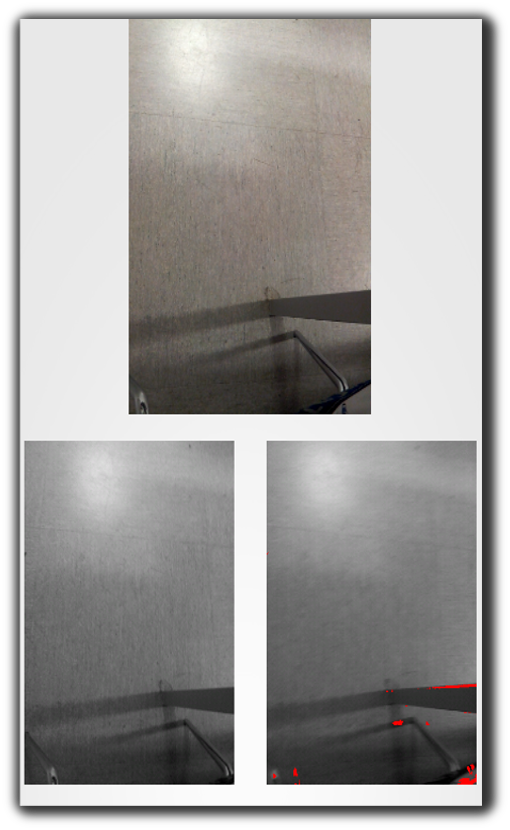
\includegraphics[scale=.18]{./img/camera.png}
\end{minipage}\begin{minipage}[c]{.65\textwidth}
\begin{itemize}
  \item In alto viene fornito lo stream di immagini catturate dalla fotocamera (anche di quelle non processate)
  \item In basso a sinistra viene visualizzata la penultima immagine processata
  \item In basso a destra viene visualizzata l'ultima immagine processata in cui vengon evidenziate in rosso le zone in cui è stato determinato movimento
\end{itemize}
\end{minipage}
\end{frame}


\section{Rilevamento rumore ambientale}
\begin{frame}
\frametitle{Microfono}
\begin{block}{~}
Attraverso il microfono è possibile monitorare il livello di rumore presente nell'ambiente e di determinarne variazioni anomale
\end{block}
\begin{itemize}
  \item Un intruso che parla 
  \item Un intruso che produce rumori per entrare nell'abitazione
  \item ...ma non tutti i rumori sono causati da intrusi: tuoni, traffico, liti d'appartamento...
\end{itemize}
Oltre a generare allarme, il determinarsi di un livello di rumore anomalo causa la registrazione di 10 secondi di audio che saranno quindi trasmessi al server in rete
\end{frame}

\begin{frame}
\frametitle{Come viene effettuato}
\begin{enumerate}
  \item Monitoraggio:
  \begin{itemize}
    \item Viene riempito un buffer di valori campionati dal microfono
    \item Viene eseguita una media dei valori campionati per ottenere un valore che possa riassumerli tutti
    \item Si converte il valore ottenuto in decibel
    \item Si confronta il valore in decibel con la soglia di sensibilità impostata dall'utente
    \item Se si riscontra un valore anomalo viene generato l'allarme e si inizia ad acquisire l'audio da poi inviare al server predisposto
  \end{itemize}
  \item Registrazione: vengono sfruttate le strutture offerte dalle API Android per acquisire 10 secondi di audio in formato AAC
\end{enumerate}
\end{frame}

\begin{frame}
\frametitle{Formati utilizzati e rappresentazione dell'informazione}
\begin{description}
  \item[PCM 16 bit] Acquisizione nativa Android. Queste informazioni vengono memorizzate temporaneamente su un buffer da 512 valori. Usare 8 bit diminuirebbe la qualità dell'audio
  \item[decibel] l'ampiezza del segnale viene tradotto in decibels fornendo come soglia di riferimento il valore 1
    {\footnotesize\[dB_i = 10\log_{10} \left(\frac{V_i}{V_o}\right)^2\]}
  \item[AAC] formato utilizzato per registrare i 10 secondi di audio. Permette di risparmiare spazio (in prospettiva di invio del file su rete) in quanto sfrutta modello psicoacustico per la compressione
  \item[Ogg Vorbis] formato utilizzato per riprodurre l'audio acquisito qualora il browser utilizzato non supporti ACC
\end{description}
\end{frame}

\begin{frame}
\frametitle{Cosa viene proposto all'utente}
\begin{minipage}[c]{.25\textwidth}
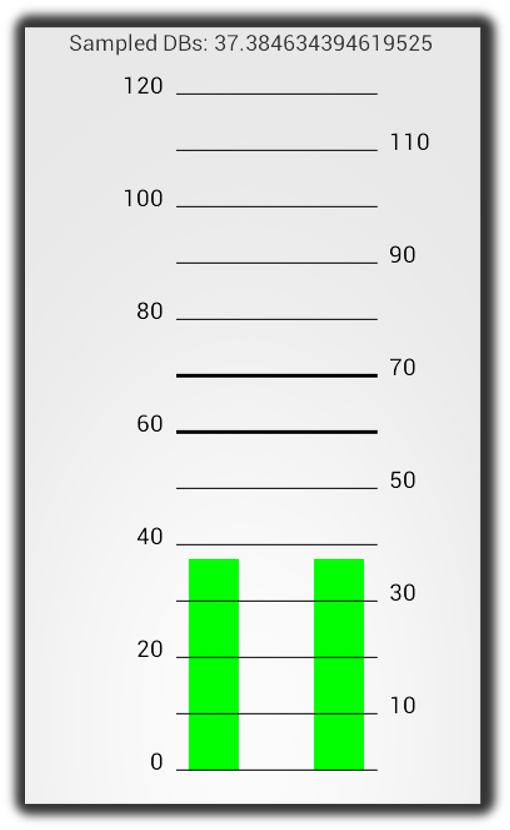
\includegraphics[scale=.18]{./img/microphone.png}
\end{minipage}\begin{minipage}[c]{.65\textwidth}
\begin{itemize}
  \item Si fornisce graficamente la media del valore campionato su scala decibel
  \item Qualora il microfono riesca a campionare audio in modalità stereo verranno visualizzati i valori di entambi i canali (ciascuna barra sarà indipendente)
  \item Vengono evidenziati due valori di soglia:
    \begin{enumerate}
      \item Il più basso rappresenta la sensibilità impostata dall'utente (è quindi il valore utilizzato per determinare un'intrusione)
      \item Il più alto è una soglia arbitraria di rumore
    \end{enumerate}
\end{itemize}
\end{minipage}
\end{frame}


\section{Invio informazioni}
\begin{frame}
\frametitle{Server remoto}
\begin{block}{~}
Si utilizza un applicazione web per poter memorizzare le informazioni raccolte dai vari dispositivi così da lasciarle sempre disponibili agli utenti
\end{block}
\begin{itemize}
  \item Il sistema di allarme è utile. \`E più utile avere a disposizione anche le informazioni da cui è scattato l'allarme
  \item Il dispositivo può essere rubato. \`E bene salvare i dati in un luogo sicuro e sempre accessibile
  \item L'applicazione non è perfetta: può determinare una falsa intrusione. Poter accedere direttamente alla informazioni catturate può evitare attacchi di panico
\end{itemize}
\end{frame}

\begin{frame}
\frametitle{Dati memorizzati}
%\begin{minipage}[c]{.2\textwidth}
\begin{center}
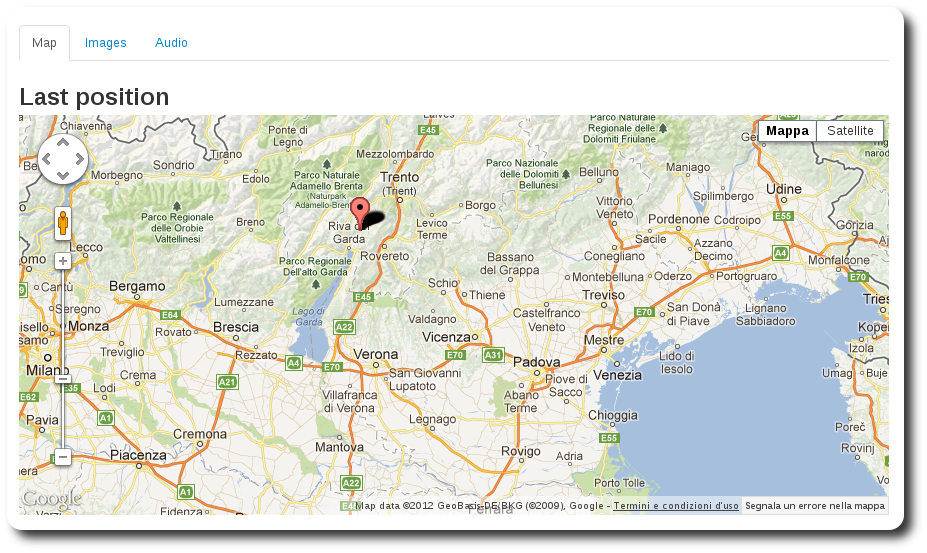
\includegraphics[scale=.15]{./img/map.png}
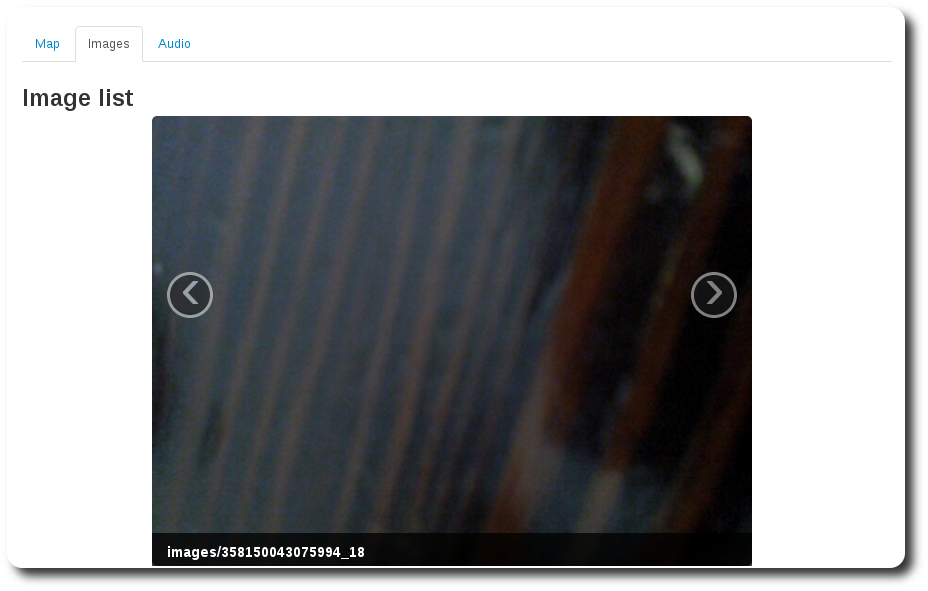
\includegraphics[scale=.15]{./img/slideshow.png}
\end{center}
%\end{minipage}\begin{minipage}[c]{.65\textwidth}
\begin{itemize}
  \item Immagini: a seconda del tipo di connessione vengono inviate 5 (3G) o 10 (WiFi) delle immagini catturate
  \item Audio: inviati i 10 secondi registrati
  \item Locazione dispositivo: ottenuta tramite GPS se attivo o tramite servizi in rete. Informazione aggiornata periodicamente
\end{itemize}
%\end{minipage}
\end{frame}

\begin{frame}
\frametitle{API REST}
\begin{block}{~}
Il server offre API REST per poter eseguire upload informazioni e per potersi autenticare: il server non accetta informazioni che potrebbero essere fasulle e si accerta che solo utenti/dispositivi autorizzati possano modificare le informazioni su server
\end{block}
\begin{itemize}
  \item Necessario essere precedentemente registrati al server
  \item Necessario un access token per eseguire upload (access token ricevuto tramite login dell'applicazione)
\end{itemize}
\texttt{~~~~\lbrack POST\rbrack  /users/accesstoken\\
~~~~\lbrack POST\rbrack	/api/phones/:phoneId/images\\
~~~~\lbrack POST\rbrack 	/api/phones/:phoneId/audio\\
~~~~\lbrack POST\rbrack  /api/phones/:phoneId/positions}


\end{frame}


\section{Bluetooth}
\begin{frame}
\frametitle{Sistema collaborativo Bluetooth}
\begin{block}{~}
Qualora non vi sia a disposizione nessuna connessione di rete ma vi sia il bluetooth attivo, si tenta di instaurare connessioni opportunistiche con altri dispositivi e di delegare a loro il compito di notificare il server dell'attuale posizione del dispositivo
\end{block}
\begin{itemize}
  \item Necessario assicurarsi che il dispositivo delegato non stia mentendo: utilizzo di un piccolo protocollo di firma digitale
\end{itemize}
\begin{center}
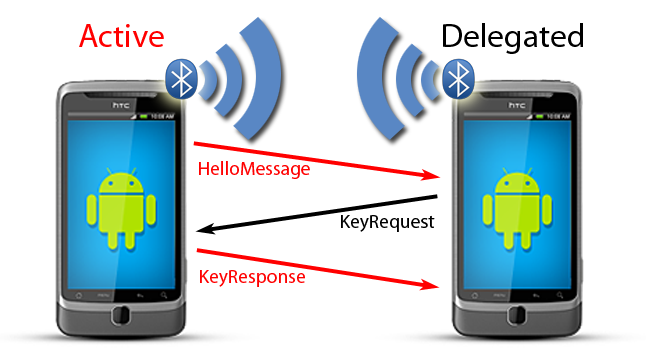
\includegraphics[scale=.2]{./img/bluetooth.png}
\end{center}
\end{frame}

\section{Conclusioni}
\begin{frame}
\frametitle{Conclusioni}
\begin{itemize}
  \item I dispositivi riescono a sopportare il carico di lavoro
  \item Meccanismi di motion detection e noise detection sono naive (potrebbero essere uilizzati concetti di image/sound processing/recognition)
  \item Protocolli di sicurezza non sono perfetti (per questioni computazionali si è deciso di non utilizzare un protocollo a chiave pubblica)
  \item Per funzionamento efficace è necessario che tanti dispositivi adottino questa applicazione (vedesi comunicazione bluetooth)
\end{itemize}
\end{frame}

\end{document}
